\documentclass{article}
\usepackage[utf8]{inputenc}
\usepackage[czech]{babel}
%\usepackage[T1]{fontenc}
\usepackage[autostyle]{csquotes}

\usepackage{graphicx}
\usepackage{amsmath}
\usepackage{amssymb}
\usepackage{geometry}
\usepackage{graphicx}
\usepackage{epstopdf}
\usepackage{caption}
\usepackage{subcaption}
\usepackage{float}
\usepackage{xcolor}
\usepackage{gensymb}
\usepackage{hyperref}
\usepackage{physics}

\captionsetup[figure]{name=Obrázek }
\captionsetup[table]{name=Tabulka }
\epstopdfsetup{outdir=./}
\geometry{a4paper, top=60pt, bottom= 50pt, left=50pt, right=50pt}
\graphicspath{ {./graphics/} }

\renewcommand{\thesection}{\arabic{section}}
\renewcommand{\refname}{Zdroje}

\title{LAR projekt}
\author{Hynek Zamazal a Jan Chleboun}
\date{}

\begin{document}
\maketitle
\section{Úvod}
Cílem projektu bylo naprogramovat robota Turtlebot tak, aby vyhledával a shazoval červené sloupky ve svém okolí aniž by se dotkl sloupku jiné barvy. Pracovali jsme v simulátoru Gazebo a robota programovali v Pythonu.
\section{Návrh}
V první fázi jsme navrhovali strukturu algoritmu. Program jsme rozdělili do několika částí:
\begin{enumerate}
    \item Main loop\\
V hlavní smyčce proběhne inicializace robota. Dále zde běží cyklus, který nejprve zadá příkaz k nalezení červeného sloupku a poté k jeho shození, případně ukončí běh celé aplikace, pokud se žádný červený sloupek nepodaří nalézt ani po důkladnějším průzkumu okolního světa.
    \item Navigator\\
    Nejrozsáhlejší část kódu. Objekt, který obsahuje pole viditelných sloupků, zvolenou cestu a cíl této cesty. Dále metody pro prohledávání světa založené na algoritmu \textit{A}* a shazování nalezených sloupků. \textit{Navigator} řídí strukturu \textit{Pilot}. 
    \item Pilot\\
    Pilot se stará o pohyb robota. Dostává rozkazy od bloku \textit{Navigator}, jakou trajektorii má sledovat.
    \item Image processing\\
    Zpracování údajů z RGB a hloubkové kamery. Hlavní je funkce \textit{process}, která najde všechny sloupky v daném obraze a přiřadí jim barvy a souřadnice relativní k robotovi.
\end{enumerate}
\section{Vidění robota}
Robot pozoruje svět kolem sebe pomocí RGB kamery a hloubkové kamery. Pomocí tzv. thresholdingu rozlišuje v RGB obraze, který převádí do HSV (Hue Saturation Value) červené, modré a zelené sloupky a také jejich stav - standing/fallen pomocí poměru šířky a výšky. Z hloubkového senzoru získá jejich vzdálenost (pokud se to z nějakého důvodu nepodaří, vypočte ji z perspektivního zkreslení) a počítá jejich souřadnice vztažené ke své pozici.
\subsection{Výpočet vzdálenosti}
Pokud z nějakého důvodu nejsou dostupná data z hloubkového senzoru, dojde k výpočtu vzdálenosti sloupku z perspektivního zkreslení šířky daného sloupku. Víme, že poloměr sloupku je $r = 2.5$ cm. Detekované okrajové pixely sloupku $\mathbf{u}_1, \mathbf{u}_2$ (v homogenních souřadnicích) převedeme na paprsky pomocí vzorce
$$\frac{1}{\lambda_i} \mathbf{x}_i = K^{-1} \mathbf{u}_i$$
Dále vypočteme úhel $\alpha$, který tyto dva paprsky svírají
$$\cos{\alpha} = \frac{\frac{1}{\lambda_1 \lambda_2}}{\frac{1}{\lambda_1 \lambda_2}}\frac{\mathbf{x}_1 \mathbf{x}_2}{\norm{\mathbf{x}_1} \norm{\mathbf{x}_2}}$$
Z tohoto úhlu spočítáme vzdálenost $z$ sloupku jako
$$z = \frac{r}{\sin{\frac{\alpha}{2}}}$$
Tento výpočet vychází z \cite{prezentace}
\subsection{Převod souřadnic}
Souřadnice v obraze v pixlech spárované se vzdáleností převádíme na souřadnice v milimetrech relativní k robotovi. Nejprve souřadnice středu sloupku v pixelech převedeme na homogenní souřadnice (jen na konec vektoru souřadnic přidáme 1). Dále pomocí matice $\mathbf{K}_{RGB}$, kterou získáme interní funkcí Turtlebot class, přepočítáme pixelové souřadnice na souřadnice v milimetrech vůči kameře. To uděláme pomocí rovnice
$$\mathbf{u}_{cam} = \mathbf{K}_{RGB}^{-1} (\mathbf{u}_{hom} \cdot z),$$
kde $\mathbf{u}_{cam}$ jsou souřadnice vůči kameře, $\mathbf{u}_{hom}$ jsou homogenní souřadnice a z je vzdálenost získaná z hloubkové kamery, nebo vypočtená z regrese.
Spočítané souřadnice poté převedeme na souřadnice vztažené k robotovi následovně
$$\mathbf{u}_{robot} = \mathbf{T} \mathbf{u}_{cam},$$
kde $\mathbf{u}_{robot}$ jsou souřadnice vztažené k robotovi, $\mathbf{u}_{cam}$ jsou souřadnice vztažené ke kameře převedené do homogenních souřadnic (pomocí přidání 1 na konec vektoru souřadnic) a $\mathbf{T}$ je matice, pro kterou platí předpis
$$\mathbf{T} =
\begin{bmatrix}
R(\theta) & \begin{matrix}
x \\ y \\ z
\end{matrix}\\
\begin{matrix}
0 & 0 & 0
\end{matrix} & 1
\end{bmatrix},
$$
kde $R(\theta)$ je rotační matice vypočtená pomocí postupu popsaného v \cite{quaterniony} z quaternionu, který jsme získali interní funkcí Turtlebot class, a x, y, z je pozice kamery vůči robotovi, kterou také získáme interní funkcí Turtlebot class. Protože x, y, z a $R(\theta)$ se nemění, má matice $\mathbf{T}$ pevnou podobu
$$\mathbf{T} =
\begin{bmatrix}
0 & 0 & 1 & -0.087 \\
-1 & 0 & 0 & 0.013 \\
0 & -1 & 0 & 0.287 \\
0 & 0 & 0 & 1
\end{bmatrix}
$$
Přepočet souřadnic založen na \cite{prezentace}.
\subsection{Použité konstanty}
\subsubsection{Thresholding}
Pro rozpoznávání sloupků metodou thresholdingu jsme použili meze uvedené v Tabulce \ref{tab:thresholding}.
\begin{center}
\captionof{table}{Tabulka hodnot pro thresholding} \label{tab:thresholding} 
 \begin{tabular}{|c | c | c | c| c|c|c |}
 \hline
Barva & Minimální & Maximální & Minimální & Maximální & Minimální & Maximální \\
 & hue & hue & saturation & saturation & value & value\\
\hline
Červená & 0 & 15 & 35 & 255 & 25 & 255\\
\hline
Zelená & 49 & 77 & 30 & 255 & 25 & 255\\
\hline
Modrá & 107 & 135 & 30 & 255 & 25 & 255\\
\hline
\end{tabular}
\end{center}
\subsubsection{Matice \texorpdfstring{$\mathbf{K}_{RGB}$}{KRGB}}
Při programování jsme narazili na bug Turtlebot class, který způsobil, že při inicializaci Turtlebota se nepodařilo získat matici $\mathbf{K}_{RGB}$, kterou potřebujeme pro přepočítávání souřadnic. Protože se však tato matice nemění, vyřešili jsme problém přidáním defaultní matice  $\mathbf{K}_{RGB}$, která se použije místo matice poskytované Turtlebot class. Tato matice je rovna:
$$
\mathbf{K}_{RGB} = 
\begin{bmatrix}
554.25469119 & 0 & 320.5 \\
0 & 554.25469119 & 240.5 \\
0 & 0 & 1
\end{bmatrix}
$$
\section{Navigace}
K plánování trasy se používá algoritmus \textit{A*}. Aby bylo plánování jednodušší, program si rozdělí plochu na jednotlivé body vzdálené od sebe 20 cm a z každého tohoto bodu může dojet pouze do 7 jeho sousedních bodů (8 sousedů - 1 ze kterého přijel). Z této množiny 7 bodů je potřeba ještě odstranit body, které jsou příliž blízko ke sloupkům, které Turtlebot nemá srazit - náš robot nepojede do stavu, který je blíže než 30 cm k jakémukoliv jinému než cílovému sloupku. Celá cesta je pak složena z úseček mezi těmito body. Cena cesty je již ujetá vzdálenost a předpokládaná cena (heuristická funkce) daného bodu je euklidovská vzdálenost od cíle.

Abychom omezili vliv nepřesnosti odometrie a detekce pozice sloupků, pokud nám \textit{A*} vrátí cestu delší než 8 kroků, ujede jich robot pouze 5 (aby si pro jistotu udržel dostatečný odstup pro identifikaci cílového sloupku z RGB obrázku), pak znovu začne hledat cílový sloupek a až ho najde, pokusí se k němu dojet. (Toto se opakuje, dokud sloupek není sražen.)

Veškerá plánovací logika robota pracuje v relativních souřadnicích - tj. z pohledu plánovájí je robot vždy v pozici $(0, 0, 0)$. (Vektor pozice je $(x, y, \theta)$, kde $\theta$ je úhel natočení.) Proto je důležité, aby před během \textit{A*} došlo k načtení sloupků z aktuálního zorného pole a vynulování odometrie. Poté se robot smí hýbat pouze podle nalezené trasy, jinak se trasa stane neplatnou, protože se změní realtivní souřadnice.

Samotné cestování podel trasy funguje následovně: Turtlebot dostane trasu jako seznam bodů \textit{(x, y)}. Sám je na začátku v bodě \textit{(0, 0)} s úhlem natočení 0. Robot se nejprve natočí směrem k bodu, do kterého má jet a poté k němu jede tak dlouho, dokud se jeho vzdálenost k tomuto cílovému bodu zmenšuje. Tento postup opakuje, dokud je od cílového bodu dál než 1 cm. Jakmile je tato podmínka splněna, přesune se robot na další bod v seznamu.

Když takto robot jezdí, používá souřadnice, které platili v místě, kde byl proveden \textit{A*} a po ujetí cesty je odometrie vynulována. Je to ekvivalentní postupu: Podívám se a zapamatuji si, kudy mám jít, abych do ničeho nenarazil. Zavřu oči, ujdu trasu a pak je znovu otevřu, abych se podíval, kam jsem se dostal a jak mám postupovat dál.

\section{Hledání cíle}
Funkce \textit{getConesFromImage()} třídy \textit{Navigator} najde sloupky v aktuálním zorném poli robota a uloží je jako seznam. (viz sekci Vidění Robota).
V případě, že Turtlebot dostane pokyn, že má hledat červený sloupek, zavolá tuto funkci. Pokud se v zorném poli červený sloupek nenachází, otočí se v protisměru hodinových ručiček o $\frac{\pi}{4}$ rad a zkusí tuto funkci zavolat znova. Otáčení a hledání sloupků opakuje, dokud na červený sloupek nenarazí. V ten okamžik k němu najde cestu a dojede ho srazit. (Viz sekci Navigace.)

Pokud ale žádný červený sloupek nenašel, otočí se robot ve směru, ve kterém poprvé viděl alespoň některé sloupky a zavolá funkci \textit{getConesFromImage()}, aby měl aktuální informace o pozicích sloupků. Poté zkontroluje, že bod \textit{(1, 0)} je dál než 50 cm od některého ze sloupků. Pokud ne, přičte k y souřadnici 20 cm a zkusí znovu zkontrolovat vzdálenost od sloupků. Toto opakuje, dokud není vzdálenost nového bodu od všech sloupků dostatečná. Turtlebot si najde cestu do tohoto nového pozorovacího bodu a dojede do něj stejným způsobem, jako kdyby jel srazit červený sloupek. Když tam dojede, znovu se začne otáčet a hledat sloupky. Tento postup se opakuje do nalezení červeného sloupku, ale maximálně 4x. Po 4 opakováních Turtlebot usoudí, že všechny červené sloupky už byly sraženy a vypne se.

Pokud ale po prvním otáčení neobjevil vůbec žádné sloupky, usoudí robot, že je jeho práce hotova a vypne se.

\section{Podpůrné aplikace}
K hlavnímu programu jsme také napsali aplikaci \textit{Threshold Picker} a \textit{Threshold Picker 2.0}, pomocí kterých můžeme nastavovat různé thresholdy pro jednotlivé barvy a pozorovat, jak to ovlivní robotovo rozpoznávání sloupků. Pohled do aplikace \textit{Threshold Picker 2.0} viz Obrázek \ref{thr_picker}.
\begin{figure}[H]
	\centering
	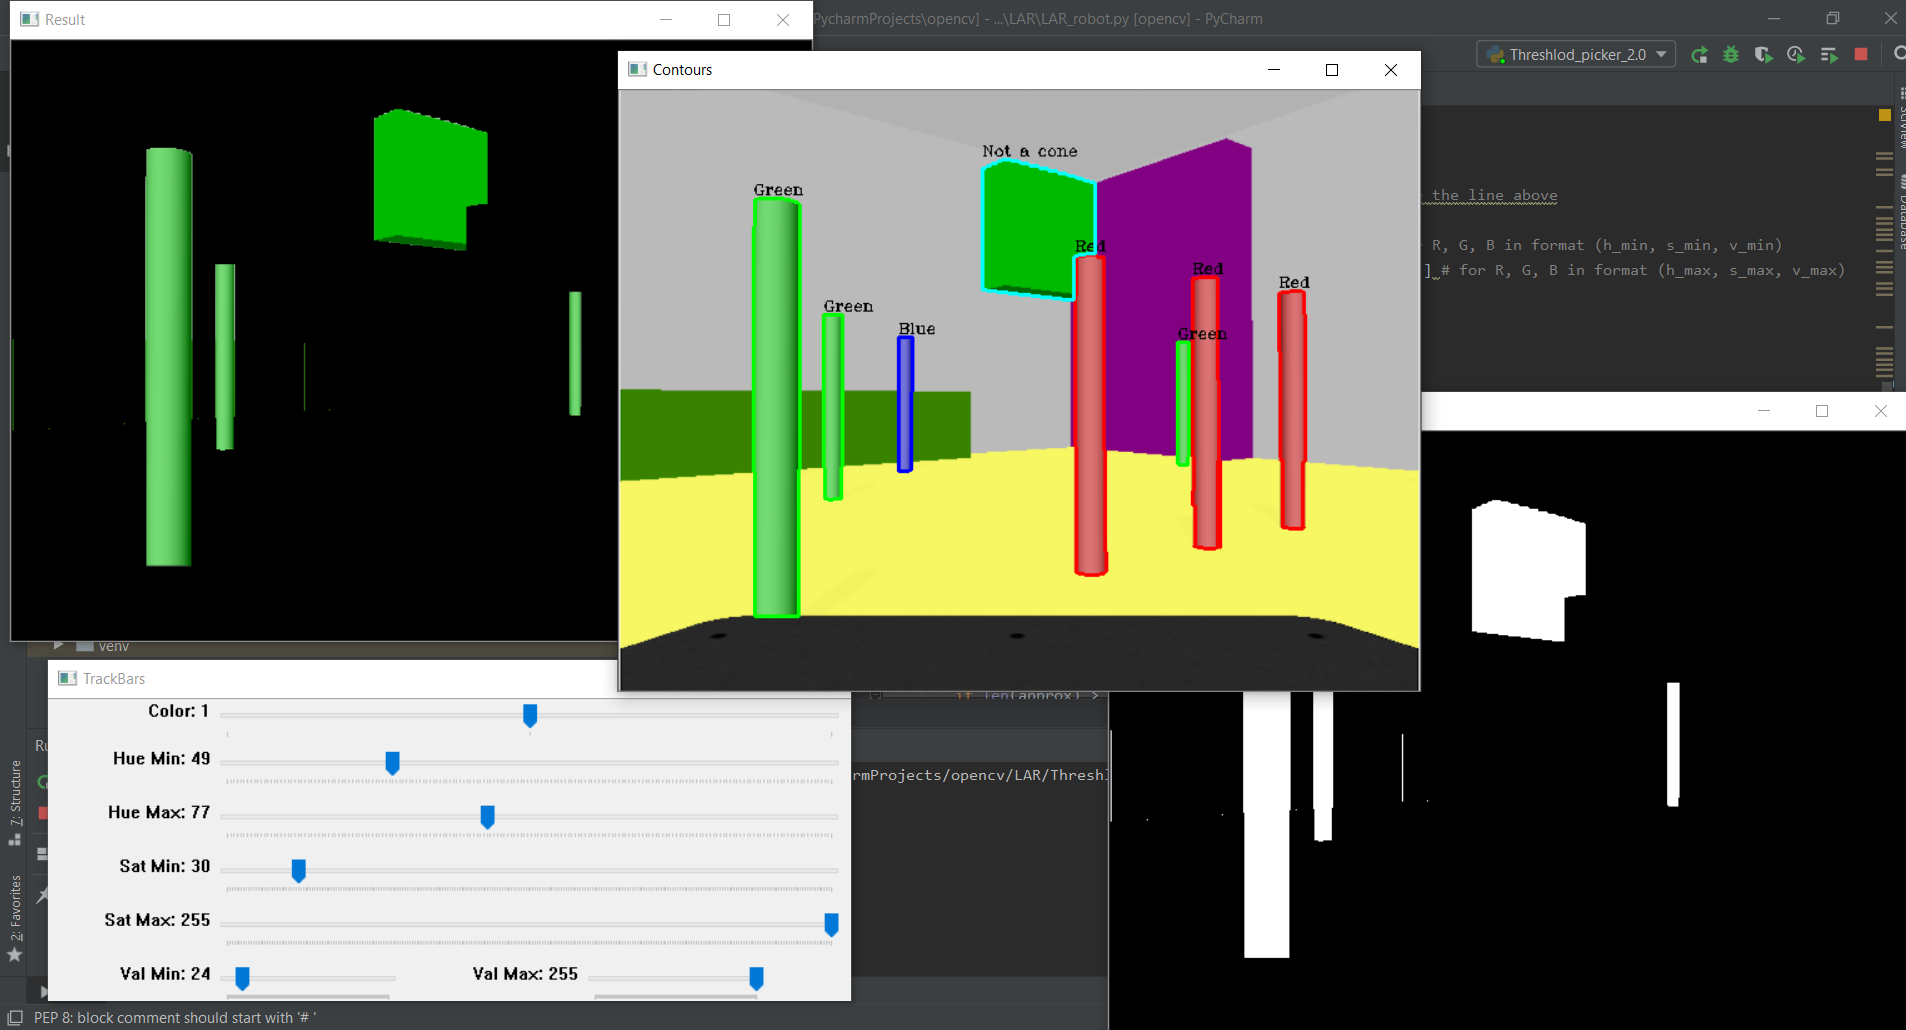
\includegraphics[scale=0.3]{Threshold_Picker.png}
	\caption{Pohled v aplikaci Threshold Picker 2.0}
	\label{thr_picker}
\end{figure}
Dalším podpůrným skriptem je skript \textit{quaternion\_to\_rot\_matrix}, který byl použit pouze jednou pro převedení quaternionu na rotační matici. Tento kód jsme převzali z \cite{quaterniony}.

\begin{thebibliography}{}

\bibitem{prezentace}
https://cw.fel.cvut.cz/wiki/\_media/courses/b3b33lar/petrik\_lar21\_en.pdf
\bibitem{quaterniony}
https://automaticaddison.com/how-to-convert-a-quaternion-to-a-rotation-matrix/
\end{thebibliography}
\end{document}


\end{document} 
